
%%%%%%%%%%%%%%%%%%%%%%%%%%%%%%%%%%%%%%%%%%%%%%%%%%

%%%%%%%%%%%%%%%%% APPENDICES %%%%%%%%%%%%%%%%%%%%%

\appendix

\section{Tidal torque \& Equations of motion}
\label{app:eom}

In this appendix, we derive the equations of motion used to simulate the asteroid angular velocity during the encounter. In particular, we describe our coordinates (section \ref{sec:coordinates}) for an encountering asteroid's position and orientation, and we parametrize its density distribution via its density moments (section \ref{sec:moments}). Then we derive an arbitrary-order equation for tidal torque (section \ref{sec:tidal-torque}) and write the equations of motion for the system (section \ref{sec:eom}). We do not consider any third-body perturbations, and we assume that the body being encountered (the central body, e.g.~a planet) is much more massive than the asteroid.

\subsection{Coordinates}
\label{sec:coordinates}

We make use of two frames of reference to model this system. One is the ``inertial frame,'' with axes denoted by $\unit{X}$, $\unit{Y}$, $\unit{Z}$ and origin placed at the central body's centre of mass. $\unit{X}$ points from the central body to the asteroid periapse, and $\unit{Z}$ points parallel to the orbit angular momentum. We assume that the mass distribution of the central body is known in this inertial frame.

Our second frame is the ``body-fixed'' frame, denoted by $\unit{x}, \unit{y}, \unit{z}$. Each axis in this frame is aligned with a principal axis and rotates with the asteroid, with its origin at the asteroid's centre of mass. For definiteness, we define $\unit{z}$ to be the principal axis with maximal MOI (this is the short axis mode, to use the vocabulary of Ref.~\cite{kaasalainen2001interpretation}). In general, we use capital letters to denote vectors in the inertial frame and lowercase vectors to denote vectors in the body-fixed frame.

The difference between the origins of the body-fixed and inertial frames is the position of the asteroid. We represent the relative orientations by $z-y-z$ Euler angles $\alpha$, $\beta$, and $\gamma$, such that a matrix $M$ rotating from the body-fixed to the inertial frame ($M\bm{r} = \bm{R}$) is given by
\begin{equation}
M = R_z(\alpha) R_y(\beta) R_z(\gamma).
\label{eqn:euler-angles}
\end{equation}
Here, $R_i(\theta)$ is a rotation around the unit vector $i$ by $\theta$ (figure \ref{fig:euler-angles}).

\begin{figure}
    \centering
    \begin{tikzpicture}
    \draw[-{Latex[length=3mm]}] (0, 0) -- (-4, 0) node[anchor=east] {$\unit x$};
    \draw[-{Latex[length=3mm]}] (0, 0) -- (2, -3) node[anchor=west] {$\unit y$};
    \draw[-{Latex[length=3mm]}] (0, 0) -- (0, 4) node[anchor=south] {$\unit z$};
    \draw[dashed, -{Latex[length=3mm]}] (0, 0) -- (3.7, -2) node[anchor=north] {};
    \draw[line width=0.5mm,-{Latex[length=3mm]}] (0, 0) -- (-0.5, -3) node[anchor=north] {$\unit X$};
    \draw[line width=0.5mm,-{Latex[length=3mm]}] (0, 0) -- (4, 1) node[anchor=south] {$\unit Y$};
    \draw[line width=0.5mm,-{Latex[length=3mm]}] (0, 0) -- (-1.6, 2.7) node[anchor=south] {$\unit Z$};
    \draw[->] (0.5, -0.75) arc (290:302:2.5);
    \draw (0.9, -0.9) node[anchor=center] {$\alpha$};
    \draw[->] (0, 1.2) arc (130:161:1.3);
    \draw (-0.3, 1.3) node[anchor=center] {$\beta$};
    \draw[->] (0.97, -0.52) arc (330:368:1.3);
    \draw (1.4, -0.25) node[anchor=center] {$\gamma$};
    %\draw[-{Latex[length=3mm]}] (0, 0) -- (0, 4) node[anchor=south] {$\unit Z$};
    %\draw[-{Latex[length=3mm]}] (0, 0) -- (4, 0) node[anchor=west] {$\unit Y$};
    %\draw[-{Latex[length=3mm]}] (0, 0) -- (-2, -2) node[anchor=east] {$\unit X$};
    \end{tikzpicture}
    \caption{$z-y-z$ Euler angles used in this work to express the orientation of the asteroid. Orientation is expressed as a rotation from the body-fixed axes (lowercase) to the inertial axes (bold lines and uppercase). The origins are co-located for demonstration purposes.}
    \label{fig:euler-angles}
\end{figure}


\subsection{Density moments}
\label{sec:moments}

The un-normalized spherical harmonics are defined as $Y_{\ell m}(\theta, \phi) = P_{\ell m}(\cos \theta)e^{im\phi}$, where $P_{\ell m}$ are the associated Legendre Polynomials without the Condon-Shortley phase. The regular and irregular spherical harmonics are further defined as
\begin{equation}
  \begin{split}
    S_{\ell m}(\bm r) &= (-1)^m (\ell - m)! \frac{Y_{\ell m}(\unit r)}{r^{\ell+1}} \\
    R_{\ell m} (\bm r) &= (-1)^m \frac{r^\ell}{(\ell + m)!} Y_{\ell m}(\unit r).
  \end{split}
\end{equation}
These spherical harmonics obey many useful identities summarized in Ref.~\cite{Gelderen1998TheSO}, which are also useful for quantum mechanics. They were used to define the density moments in equation \ref{eqn:klm}, which can be extended to the central body:
\begin{equation}
  \begin{split}
    &J_{\ell m} = \frac{a_\mathcal{B}^{2-\ell}}{I_\mathcal{B}} \int_\mathcal{B} d^3 r \rho_\mathcal{B}(\bm r) R_{\ell m}(\bm r)\\
  \end{split}
  \label{eqn:jlm}
\end{equation}
By contrast, $J_{\ell m}$ should be computed in the inertial frame. The length scale $a_\mathcal{B}$ and MOI scale $I_\mathcal{B}$ can be defined similarly to $a_\mathcal{A}$ and $a_\mathcal{B}$ in equations \ref{eqn:aa} and \ref{eqn:ia}, but they could also be set to any other scales of the same units, e.g. $a_\mathcal{B}$ equal to the central body radius and $I_\mathcal{B} = \mu_\mathcal{B}a_\mathcal{B}^2$, where $\mu_\mathcal{B}$ is the central body mass.

Note that both $J_{\ell m}$ and $K_{\ell m}$ are unitless. We call them ``moments'' because the $R_{\ell m}(\bm r)$ contains an $r^\ell$ dependence so that $K_{\ell m}$ is the $\ell$th density moment of the asteroid.

These moments share several key properties which we discuss before continuing. Firstly, for real mass density, properties of the spherical harmonics imply that $K_{\ell m} = (-1)^m K_{\ell, -m}^*$. Therefore, the set of $K_{\ell m}$ for $\ell < \ell_\text{max}$ contains $\ell_\text{max}^2$ degrees of freedom. However, some of these degrees of freedom are redundant with the choice of coordinates: $K_{1m} = 0$ since the body-fixed frame is centred on the asteroid centre of mass. Further calculation reveals that the alignment of the body-fixed frame with the asteroid principal axes also forces $K_{21}= 0$ and $\Im K_{22}=0$. The only physical density moments for $\ell \leq 2$ are therefore $K_{22}$, $K_{20}$, and $K_{00}$. The first two are related to the MOI around each principal axis by equation \ref{eqn:moi}, while $K_{00} = \mu_\mathcal{A} a_\mathcal{A}^2 / I_\mathcal{A}$ will not be relevant to this study as it does not appear in equation \ref{eqn:tidal-torque}. 

The physical meaning of $K_{22}$ and $K_{20}$ can also be interpreted via a special case: if the asteroid is a uniform-density triaxial ellipsoid, the moments of inertia are simple to compute in terms of the semi-axis lengths and can be compared to those found in equation \ref{eqn:moi}. This yields semi-axis lengths of 
\begin{equation}
  \begin{split}
  a &= \sqrt{\frac{5}{3}}a_\mathcal{A}\sqrt{1-2K_{20}+12K_{22}}\\
  b &= \sqrt{\frac{5}{3}}a_\mathcal{A}\sqrt{1-2K_{20}-12K_{22}}\\
  c &= \sqrt{\frac{5}{3}}a_\mathcal{A}\sqrt{1+4K_{20}}.
  \label{eqn:ellipsoid-axes}
  \end{split}
\end{equation}
The higher-order moments $K_{3m}$ can be thought of loosely as measuring the large-scale asymmetries of the asteroid. An asteroid that is mirror-symmetric along the $\unit{x}$ axis (meaning $\rho_\mathcal{A}(x,y,z)=\rho_\mathcal{A}(-x,y,z)$) necessarily sets certain density moments to zero. Which density moments are zeroed by which mirror symmetries is outlined in table \ref{tab:klm-symmetries}. All $K_{3m}$ are zeroed by at least one mirror symmetry. 

\begin{table}
  \centering
  \begin{tabular}{c|ccccccc}
    \hline
    $\ell$ & $\Re K_{\ell 3}$ & $\Im K_{\ell 3}$ & $\Re K_{\ell 2}$ & $\Im K_{\ell 2}$ & $\Re K_{\ell 1}$ & $\Im K_{\ell 1}$ & $K_{\ell 0}$ \\ \hline
    0 &  &  &  &  &  &  & -\\ 
    1 &  &  &  &  & x & y & z\\ 
    2 &  &  & - & x,y & y,z & x,z & -\\ 
    3 & x,z & y,z & z & x,y,z & x & y & z\\ \hline
  \end{tabular}
  \caption{Axes of mirror symmetry that imply zeroed density moments. For example, for mirror symmetries along $\unit y$ or $\unit z$, $\Im K_{32}=0$. Mirror symmetry along $\unit x$ means $\rho_\mathcal{A}(x, y, z) = \rho_\mathcal{A}(-x, y, z)$. Dashes indicate that none of the mirror symmetries zero the moment in question. Since $r^2>0$ for $r\neq 0$, no symmetries set $a_\mathcal{A}=0$ either.}
  \label{tab:klm-symmetries}
\end{table} 

Finally, the requirement that $\rho_\mathcal{A}(\bm r) \geq 0$ everywhere restricts $K_{\ell m}$. In the case of $K_{2m}$, this fact and the constraint that $I_z$ is larger than $I_x$ or $I_y$ requires $K_{20}$ and $K_{22}$ to fall in the triangle
\begin{equation}
  -\frac{1}{4} \leq K_{20} \leq 0, \qquad |K_{22}| \leq -\frac{K_{20}}{2}.
  \label{eqn:parameter-bounds}
\end{equation}
An analytical constraint on $K_{3m}$ based on this property is more difficult to derive, but in practice, we also observe that $|K_{3m}| < 0.01$.




\subsection{Tidal torque}
\label{sec:tidal-torque}

Derivations for the tidal torque experienced by a rigid body in the gravitational field of a larger mass have been computed by several previous studies \cite{paul88,HouMar2017,BOUE2009750, ashenberg07}, often in terms of the MOI of the rigid body (or higher order moments of inertia), and to varying degrees of precision. A simple, first-order derivation is also easily computable in terms of the asteroid MOI in the inertial frame.

Here, we present a new derivation of the tidal torque to arbitrary orders in terms of the density moments of an asteroid defined in section \ref{sec:moments}. These density moments can be pre-computed and do not have to be re-evaluated every time-step.

Throughout this paper, we assume that the asteroid remains rigid throughout the encounter. We also assume no third-body perturbations from other Solar System objects. (More accurately, we assume that all third-body perturbing objects lie closer to the central body's centre of mass than the asteroid perigee distance so that their density moments can be included in the density moments of the central body.) For the sake of simplicity, we also assume that the density moments of the central body are known and do not evolve with time (i.e., the central body's rotation is marginal compared to the timescale of the encounter).

The gravitational potential energy of the central body is, in its most general form,
\begin{equation}
V(\bm R') = -G\int_\mathcal{B} d^3 R \rho_\mathcal{B}(\bm R) \frac{1}{|\bm{R}-\bm{R'}|}.
\label{eqn:first-pe}
\end{equation}
where $\rho_\mathcal{B}$ is the density distribution of the central body and $\mathcal{B}$ indicates the central body's volume. All vectors here are written in the inertial frame. Given $|\bm{R}| < |\bm{R'}|$, Ref.~\cite{Gelderen1998TheSO} gives the identity
\begin{equation}
  \frac{1}{|\bm R - \bm R'|} = \sum_{\ell, m} R_{\ell m}(\bm R) S_{\ell m}^*(\bm R'),
  \label{eqn:ylm-expansion}
\end{equation}
where the sum is shorthand for $\sum_{\ell, m} = \sum_{\ell = 0}^\infty \sum_{m=-\ell}^\ell$.
We are interested in translating the potential energy of equation \ref{eqn:first-pe} to the body-fixed frame. To do this, we let $\bm{R'} = \bm D + \bm U$, where $\bm D$ is the location of the asteroid in the inertial frame. We further define $\bm U = M\bm u$, where $\bm u$ is in the body-fixed frame and $M$ is the rotation matrix given by the Euler angles $\alpha$, $\beta$, and $\gamma$ (see section \ref{sec:coordinates}). The translation from $\bm {R'}$ to $\bm U$ is then attained by the identity 
\begin{equation}
  S_{\ell m}(\bm R') = \sum_{\ell', m'} (-1)^{\ell'}R^*_{\ell' m'}(\bm U)S_{\ell+\ell', m + m'} (\bm D),
  \label{eqn:ylm-translation}
\end{equation}  
provided by Ref.~\cite{Gelderen1998TheSO}, and from $\bm U$ to $\bm u$ is given by
\begin{equation}
  \begin{split}
    Y_{\ell m}(M\bm u) = \sum_{m'=-\ell}^\ell & (-1)^{m+m'}\sqrt{\frac{(\ell-m')!(\ell+m)!}{(\ell+m')!(\ell-m)!}} \\
    & \times \mathcal{D}^\ell_{mm'}(M)^* Y_{\ell m'}(\bm u).\\
  \end{split}
  \label{eqn:ylm-rotation}
\end{equation}
Here, $\mathcal{D}^\ell_{mm'}(M)$ are the Wigner-$D$ matrices, which are determined by the Euler angles $\alpha$, $\beta$, and $\gamma$ of $M$.

Equations \ref{eqn:first-pe} to \ref{eqn:ylm-rotation} then provide formula for $V(\bm u)$ expressed as a sum of integrals over $\mathcal{B}$ of the central body density $\rho_\mathcal{B}(\bm R)$ times $R_{\ell m}(\bm R)$. These are expressed via equation \ref{eqn:jlm} as $J_{\ell m}$.

The tidal torque experienced by the asteroid (in the body-fixed frame) is given by
\begin{equation}
  \bm{\tau}(\bm u) = \int_\mathcal{A} d^3 u \rho_\mathcal{A}(\bm u) (\bm u \times (-\nabla_{\bm u} V(\bm u)))
\end{equation}
where $\rho_\mathcal{A}$ is the density distribution of the asteroid and $\mathcal{A}$ indicates the volume of the asteroid. Making use of one more identity concerning the derivatives of spherical harmonics:
\begin{equation}
  \begin{split}
  \bm u \times \nabla R_{\ell m}(\bm u)=&\frac{1}{2}\Big[(i\unit x - \unit y)(\ell-m+1)R_{\ell,m-1}(\bm u)\\
  &+(i\unit x+\unit y)(\ell+m+1)R_{\ell,m+1}(\bm u)\\
  & +2im\unit z R_{\ell m}(\bm u)\Big],
  \end{split}
\end{equation}
tidal torque can now be expressed as a function only of the constants $J_{\ell m}$, $K_{\ell m}$, $a_\mathcal{A/B}$, $I_\mathcal{A/B}$, and the asteroid orientation and position (equation \ref{eqn:tidal-torque}). Some $K_{\ell m}$ terms are written in this equation with $|m|>\ell$; these should all be taken to be zero.

Equation \ref{eqn:tidal-torque} possesses a few explicit properties. Firstly, $\bm \tau$ is independent of asteroid mass. The mean density of the asteroid is therefore not constrained by tidal torque analysis. Secondly, torque is largest when $D$ is small (as expected), with the leading order of $\bm \tau$ proportional to $D^{-3}$. Thirdly, each $J_{\ell m}K_{\ell' m'}$ term is multiplied by $(a_\mathcal{B}/D)^\ell (a_\mathcal{A}/D)^{\ell'}$, the latter of which especially is small in most cases. Equation \ref{eqn:tidal-torque} can therefore be computed approximately by removing terms of large $\ell$ and $\ell'$. For our analysis, we removed $\ell' > 3$ and we usually keep only $\ell=0$. Note that $\ell=1$ contributes nothing since $J_{1m}=0$. $J_{2m}$ measures the oblateness and its effects are studied in appendix \ref{app:uncertainty-dependence}.

Further insight can be gained by remarking the value of the first-order of $\bm \tau$ for particular Euler angle cases. Setting $\beta = 0$ produces diagonal Wigner-$D$ matrices, and hence $\bm \tau \parallel \unit z$ to first-order. This $\beta=0$ condition is equivalent to $\unit z \parallel \unit Z$ (see figure \ref{fig:euler-angles}).

For $\beta = \pi/2$, there are two interesting cases. One is for $\alpha = \phi$ (or $\alpha = \pi + \phi$), where $\phi$ is the angle between the asteroid and the perigee. In this case, $\bm \tau = 0$ to first-order. The second case is $\alpha = \phi \pm \pi/2$, when again $\bm \tau \parallel \unit z$. At perigee ($\phi=0$), these conditions are equivalent to $\unit z \parallel \unit X$ and $\unit z \parallel \unit Y$ respectively.

The $\bm \tau \parallel \unit z$ cases are interesting because they do not induce tumbling. If velocity is $\bm \omega \parallel \unit z$ (a non-tumbling state, since $\unit z$ is a principal axis), then $\bm \omega \parallel \bm L$ and $\bm \tau = \dot{\bm L} \parallel \dot{\bm \omega}$ so that $\bm \omega$ remains parallel to $\unit z$ and non-tumbling. These cases of torque are additionally significant because not as many terms contribute to $\tau_z$ as to $\tau_x$ and $\tau_y$.

\subsection{Equations of motion}
\label{sec:eom}


The equations of motion of the asteroid position $\bm D$ are given by Newton's law of gravitation
\begin{equation}
  \dot{\bm V} = -\frac{G \mu_\mathcal{B}}{D^3} \bm D \qquad \dot{\bm D} = \bm V
  \label{eqn:pos-eom}
\end{equation}
where $\bm V$ is the asteroid velocity in the inertial frame. Rather than derive equations of motion for the Euler angles (which suffer from gimbal lock), we instead represent the orientation of the asteroid with a quaternion $\quat q$ which can be converted into Euler angles to compute $\mathcal{D}(\alpha, \beta, \gamma)$. This quaternion evolves as 
\begin{equation}
  \dot{\quat q} = \frac{1}{2}\quat q\quat \omega.
  \label{eqn:quat-eom}
\end{equation}
for angular velocity $\bm \omega$ given in the body-fixed frame. The equations of motion of $\bm \omega$ in turn are given by
\begin{equation}
  \begin{split}
    I_x \dot \omega_1 - \omega_y \omega_z (I_y - I_z) &= \tau_x\\
    I_y \dot \omega_2 - \omega_z \omega_x (I_z - I_x) &= \tau_y\\
    I_z \dot \omega_3 - \omega_x \omega_y (I_x - I_y) &= \tau_z.
  \end{split}
  \label{eqn:omega-eom}
\end{equation}
Equations \ref{eqn:tidal-torque}, \ref{eqn:moi}, and \ref{eqn:pos-eom} to \ref{eqn:omega-eom} form a set of non-linear, first-order coupled differential equations in which can be numerically integrated. They are expressed in terms of the constant physical parameters $I_\mathcal{A/B}$, $a_\mathcal{A/B}$, $J_{\ell m}$, and $K_{\ell m}$.





\section{Additional density distribution models}
\label{app:more-models}

Two models were discussed in section \ref{sec:density-distro} to translate density moment constraints into density distribution constraints. Here we outline two additional models, the nearly-uniform and the harmonic models, which are less conventional but still useable for extracting density distribution properties. Unlike the finite element and lumpy models discussed in the main text, these models will yield smooth distributions with no discrete transitions. They also rely on a known surface for the asteroid.

\subsection{Nearly-uniform model}
In this ``nearly-uniform'' model, we seek to pick one density distribution from the many distributions consistent with the data by maximizing a prior distribution $f[\rho(\bm r)]$, which can be chosen manually. Any prior distribution can be chosen, but the following prior is both interesting and numerically efficient.

As part of our prior, we require that the asteroid density distribution satisfy $I_\mathcal{A} = \mu_\mathcal{A} a_\mathcal{A}^2$. This constraint is desirable as it is obeyed for uniform density distributions. To define the prior, we divide the asteroid into $n \gg 1$ small regions of volume $V$, each with position $\bm r_i$ and density $\rho_i = \delta_i + 1$. Setting the mass of the asteroid equal to its volume, the average density is 1, so $\delta_i$ is the difference between the average and local density. We set $f[\rho(\bm r)]$ to be a multivariate-Gaussian distribution on $\delta_i$, centred on zero to minimize non-uniformity, i.e.
\begin{equation}
  f[\rho(\bm r)] \propto \prod_i \exp\parens{-\frac{\delta_i^2}{2\sigma^2}} \implies \ln f[\rho(\bm r)] \simeq -\sum_i \delta_i^2
  \label{eqn:nu-f}
\end{equation}
where $\sigma$ is an irrelevant constant. The density moments, MOI scale, and mass are 
\begin{equation}
  K_{\ell m} = \frac{V}{\mu_\mathcal{A}a_\mathcal{A}^{\ell}} \sum_i (\delta_i + 1) R_{\ell m}(\bm r_i)
  \label{eqn:nu-klm}
\end{equation}
\begin{equation}
  I_\mathcal{A} = \mu_\mathcal{A} a_\mathcal{A}^2 = V \sum_i (\delta_i + 1) r_i^2
  \label{eqn:nu-ia}
\end{equation}
\begin{equation}
  \mu_\mathcal{A} = V\sum_i (\delta_i + 1) \implies 0 = \sum_i \delta_i.
  \label{eqn:nu-mass}
\end{equation}
Writing $\delta_i$ as an $n$-dimensional vector $\bm \delta$, equation \ref{eqn:nu-klm} is a matrix equation for $K_{\ell m}$, and equations \ref{eqn:nu-ia} and \ref{eqn:nu-mass} are vector dot product equations. Combining $K_{\ell m}$, $I_\mathcal{A}$, and $0$ into a single vector $\bm K$, these equations can be written as a single underdetermined matrix equation we denote as 
\begin{equation}
  \bm K = M \bm \delta + \bm C,
  \label{eqn:nu-matrix}
\end{equation}
where the components of constant matrix $M$ and constant vector $\bm C$ are known given a fixed layout of the $n$ regions. Some of the components of $\bm K$, such as $I_\mathcal{A}$, $\mu_\mathcal{A}$, and $K_{1m}$, are constraints. We treat the other components as parameters of the model. The task is then to find $\bm \delta$ that satisfies equation \ref{eqn:nu-matrix} and maximizes $f(\bm \delta)$. But the form of equation \ref{eqn:nu-f} shows that the maximum of $\ln f$ (also the maximum of $f$) is the minimum of $|\bm \delta|^2$. This shortest value of $\bm \delta$ that obeys equation \ref{eqn:nu-matrix} is given by the Moore-Penrose inverse:
\begin{equation}
  \bm \delta = M^+ (\bm K - \bm C); \qquad M^+ = M^\dagger(M M^\dagger)^{-1}
  \label{eqn:nu-delta}
\end{equation}
where $M^\dagger$ is the adjoint of $M$.

The prior distribution on $\rho(\bm r)$ discussed in section \ref{sec:fit} can be implemented by individually checking the components $\bm \delta$ computed by equation \ref{eqn:nu-delta} and confirming that $1 + \delta_i$ lies within the acceptable range of densities.
 can be implemented by individually checking the components $\bm \delta$ computed by equation \ref{eqn:nu-delta} and confirming that $1 + \delta_i$ lies within the acceptable range of densities.


\subsection{Harmonic model}
This the ``harmonic model'', we limit ourselves to density distributions that are harmonic; i.e., they satisfy $\nabla^2 \rho(\bm r) = 0$. We have no physical justification for why this assumption should be true, but it is useful as a simplification to gain qualitative insight into the properties of the asteroid density distribution.

A harmonic density distribution can be expanded in terms of the spherical harmonics as $\rho(\bm r) = \sum_{\ell m} C_{\ell m} R_{\ell m}(\bm r)^*$ where $C_{\ell m}$ are complex, free parameters. This series can be truncated at some maximum $\ell$. The density moments, MOI scale, and mass can then be explicitly computed as a function of $C_{\ell m}$:
\begin{equation}
  K_{\ell m} = \frac{a_\mathcal{A}^{2-\ell}}{I_\mathcal{A}} \sum_{\ell m} C_{\ell' m'} \int_\mathcal{A} d^3 r R_{\ell' m'}(\bm r)^* R_{\ell m}(\bm r)
  \label{eqn:harmonic-klm}
\end{equation}
\begin{equation}
  I_\mathcal{A} = \sum_{\ell m} C_{\ell m} \int_\mathcal{A} d^3 r R_{\ell m}(\bm r)^* r^2
  \label{eqn:harmonic-ia}
\end{equation}
\begin{equation}
  \mu_\mathcal{A} = \sum_{\ell m} C_{\ell m} \int_\mathcal{A} d^3 r R_{\ell m}(\bm r)^*.
  \label{eqn:harmonic-mass}
\end{equation}
These integrals can be pre-computed given a known asteroid shape $\mathcal{A}$, so that computing $C_{\ell m}$ to match a given $K_{\ell m}$ is fast. Furthermore, their values when $\mathcal{A}$ is spherical gives us insight into the influence of $K_{\ell m}$ on density distributions. In this case, $I_\mathcal{A} \propto C_{00}$ and the integral of equation \ref{eqn:harmonic-klm} is non-zero only when $\ell' = \ell$ and $m'=m$. Therefore, $C_{\ell m}$ is proportional to $K_{\ell m}$. The density distribution can be immediately visualized given the density moments as a sum of the solid spherical harmonics weighted by $K_{\ell m}$. When the asteroid is non-spherical, the shape itself contributes to $K_{\ell m}$ so as to break this picture.

Imposing constraints on these moments is also necessary. The choice of mass is enforced via equation \ref{eqn:harmonic-mass}. We impose bounds on $\rho(\bm r)$ by acknowledging that harmonic functions such as $\rho(\bm r)$ in a region such as $\mathcal{A}$ attain their maxima on the boundary of the region, so that it is only necessary to ensure that $\rho$ lies within the allowed range on the asteroid boundary rather than within the entire asteroid. This can be done by parametrizing the asteroid surface as a function of two variables (e.g., latitude and longitude) and minimizing and maximizing $\rho$ with respect to those variables, ensuring these minima and maxima are within the allowed range.




\section{Reference asteroid configurations}
\label{app:reference-configs}

Except when otherwise mentioned, we use the following asteroid encounter parameters. Many of the parameter choices are made to increase the precision of observations (a close orbit, large asteroid, etc.) This is so that our methodology's output is most sensitive to changes in these parameters.

\begin{enumerate}
  \item An orbit around a spherical, Moonless Earth with $6$ km s$^{-1}$ excess velocity and perigee at 5 Earth radii. This orbit was chosen to roughly match that of Apophis. These orbital parameters correspond to an eccentricity of 3.88. 
  \item An initial roll of $\gamma_0=\pi/8$.
  \item A cadence of 2 minutes and observational uncertainty of $\sigma_\theta = 10^{-2}$ and $\sigma_P / P = 10^{-7}$.
  \item A rotational period of 9 hours, with the angular velocity vector distributed between the $\unit X$, $\unit Y$, and $\unit Z$ axes in a $1:2:-2$ ratio.
  \item An asteroid with radius $a_\mathcal{A} = 1$ km and $K_{3m}=0$. For $K_{22}$ and $K_{20}$, we use two standard values: one with $(K_{22}, K_{20}) = (0, -0.097)$ and one with $(0.052, -0.202)$. Including the third point obtained by reflection $K_{22}\rightarrow -K_{22}$, these are the three points that minimize the mean distance between an arbitrary point in the allowed parameter space (equation \ref{eqn:parameter-bounds}) and these reference values. The first point is called the symmetric case because the corresponding uniform-density-ellipsoid model is rotationally symmetric around $\unit z$. The second case and its reflection are called the asymmetric cases. Values of $(0.052, -0.202)$ have $a < b$ in the ellipsoid model, and the reflected value has $a > b$. If not specified, we use the $a < b$ case. Specifically, the asymmetric case has $a=1140$ m, $b=1839$ m, and $c=565$ m, while the symmetric case has $a=b=1411$ m and $c=1008$ m.
\end{enumerate}

The surface of a spherical asteroid with this rotational period and $a_\mathcal{A}$ rotates at $\SI{25}{\centi\meter\per\second}$ at the equator. The asymmetric and symmetric ellipsoids have maximum equatorial velocities of $\SI{36}{\centi\meter\per\second}$ and $\SI{27}{\centi\meter\per\second}$ respectively.


% \section{The cadence cut-off}
% \label{app:cadence-tests}

% \jtd{Remove this section or included it in the following section.}

% In section \ref{sec:scan-cadence}, we noted that posterior uncertainty as a function of observation cadence $\Delta t$ appears to increase suddenly near $\Delta t \sim T_\text{cad}=30-40$ min. In this appendix, we discuss the location of this cadence cut-off as a function of the physical parameters of the asteroid.

% In figure \ref{fig:cad-contour}, we display contour plots of posterior uncertainty $\sigma(K_{\ell m})$ of the fit parameters as a function of both cadence $\Delta t$ and $P_\omega$ (left panel) or the relative orbit speed $t_\text{spin} / t_\text{orbit}$ (right panel). Both panels show the same sudden increase in posterior uncertainty we named $T_\text{cad}$, located around the region where $\sigma_\rho / \rho = 100\%$ and now visible as a function of frequency and relative orbit speed. In all cases, the value of $\gamma_0$ was set so that all data points achieve the same value of $\gamma$ at perigee.

% \begin{figure*}
%   \centering
%   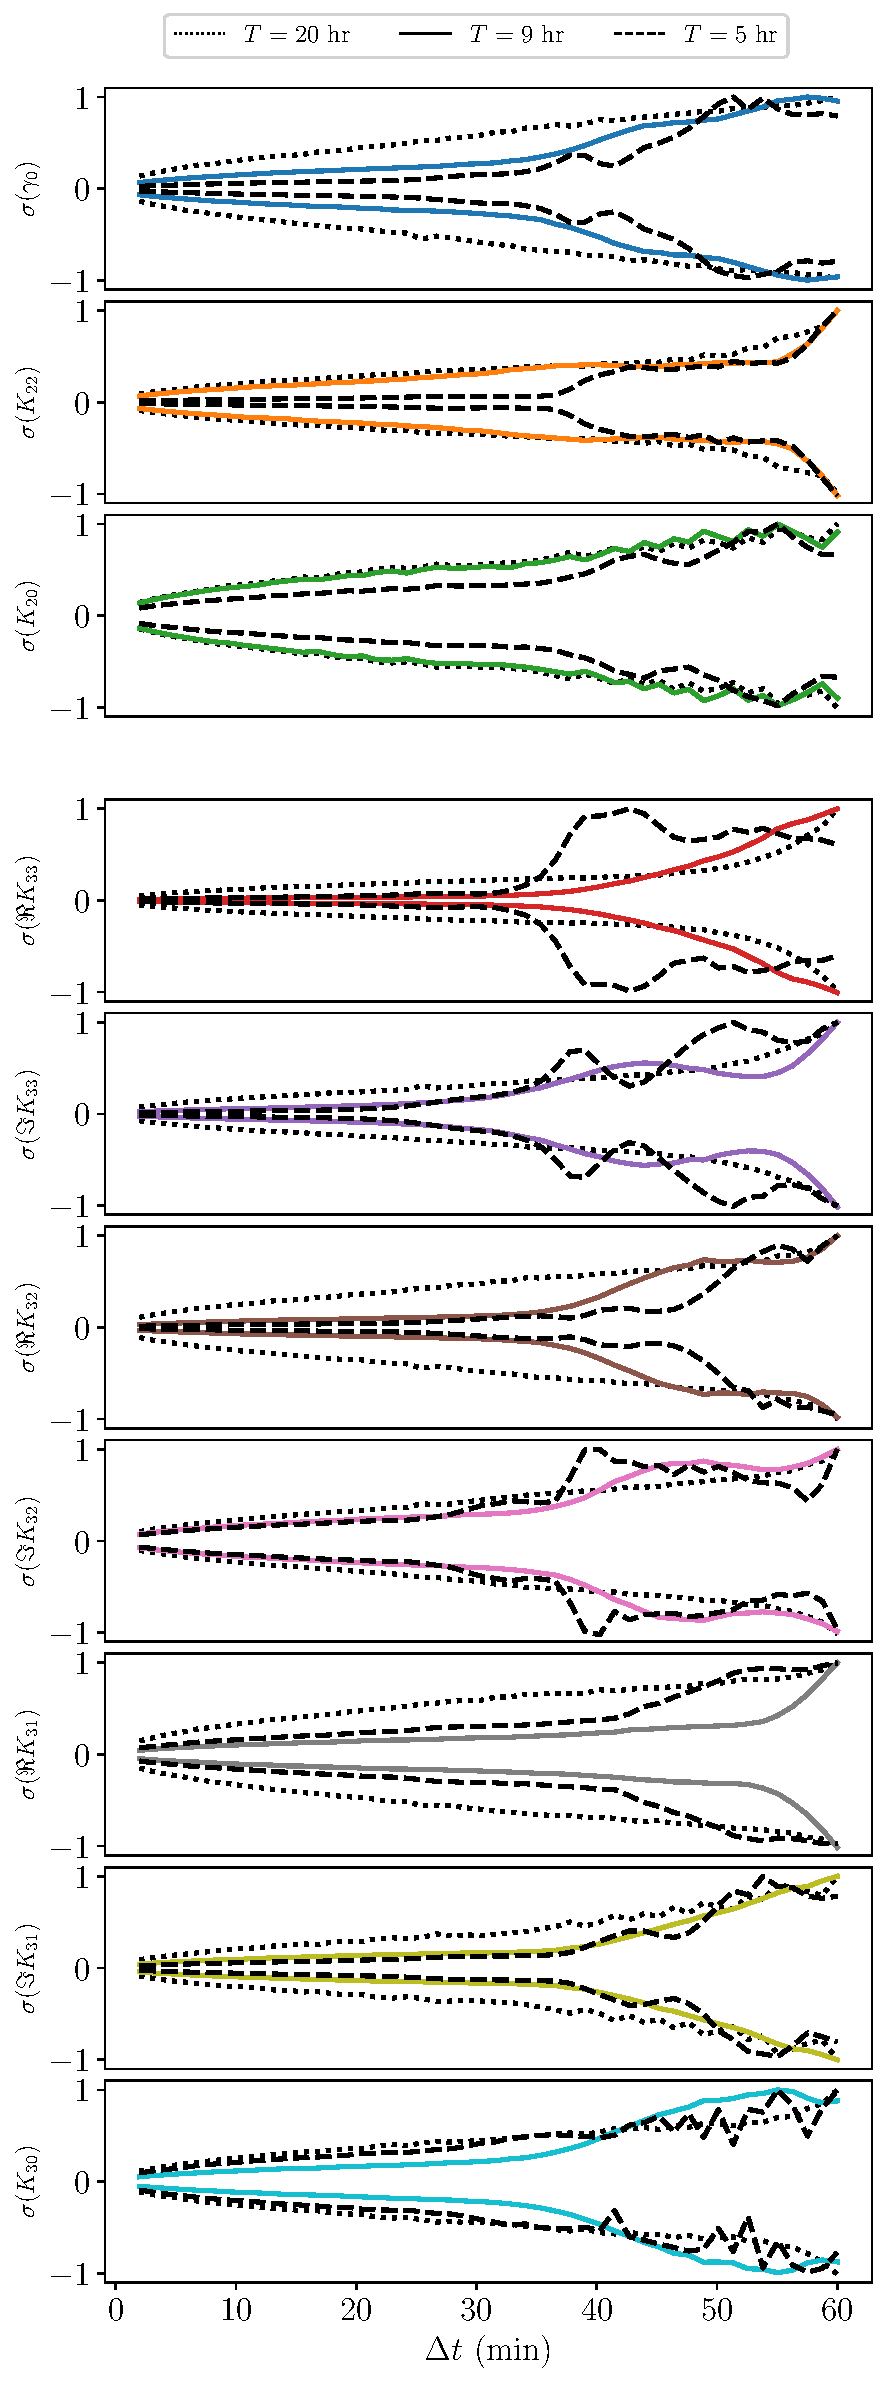
\includegraphics[width=0.48\textwidth]{figs/cad-period.pdf}\hfill
%   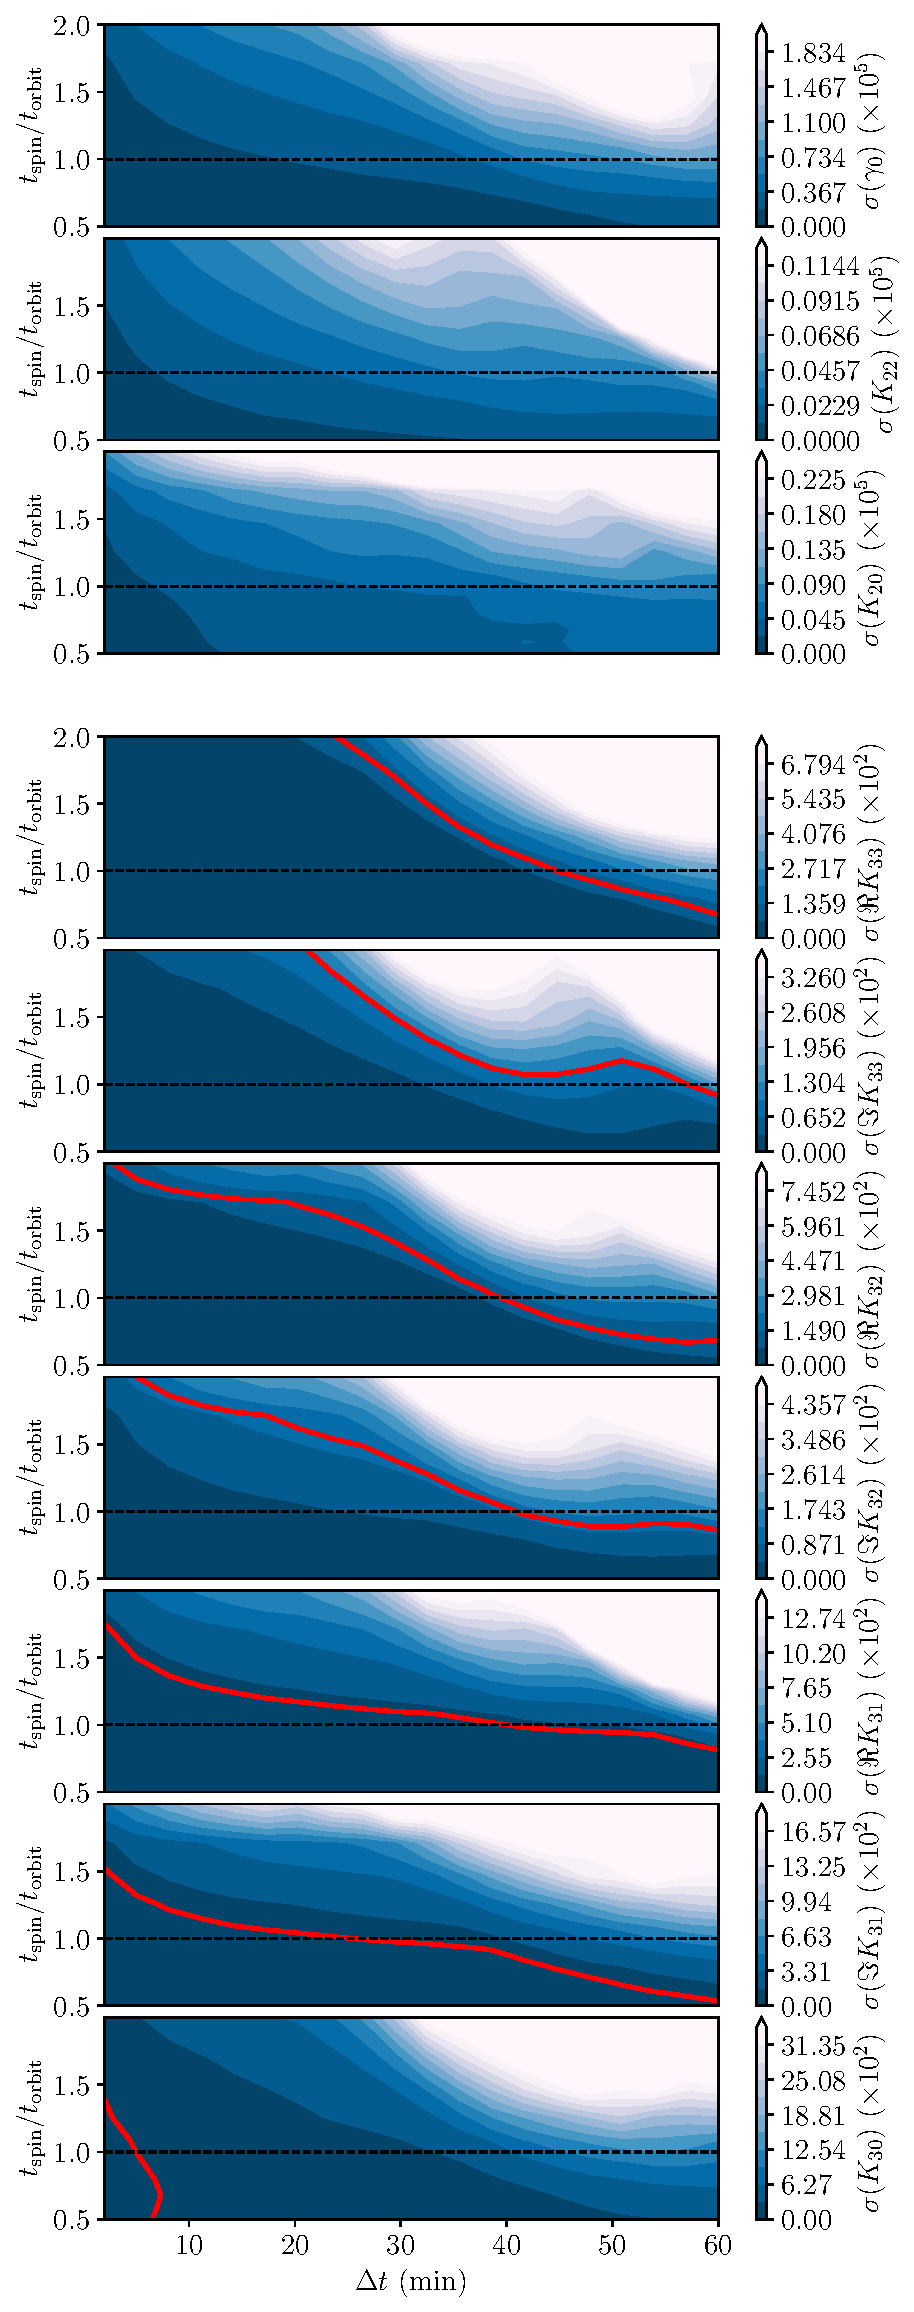
\includegraphics[width=0.48\textwidth]{figs/cad-speed.pdf}
%   \caption{Contour plots showing posterior uncertainties as a function of cadence $\Delta t$ and dynamical time scales for the encounter: rotational period $P_\omega$ (\textit{left}) and the relative speed of the orbit (\textit{right}; see text for a definition). The reference values of $P_\omega=9$ hr and $t_\text{spin}/t_\text{orbit}=1$ are shown as dotted lines. The solid (dotted) red line represents the $\sigma_\rho / \rho = 100\%$ (20\%) threshold. Cadence cut-off depends strongly on both $P_\text{omega}$ and $t_\text{spin}/t_\text{orbit}=1$.}
%   \label{fig:cad-contour}
% \end{figure*}

% Figure \ref{fig:cad-contour} demonstrates that large rotational period produces high $T_\text{cad}$. The dependence on $P_\omega$ agrees with the fact that large rotational periods for fixed cadence lead to better posterior uncertainty, discussed in section \ref{sec:scan-period}. The figure also demonstrates that for large $P_\omega$, $T_\text{cad}$ depends less strongly on $P_\text{omega}$ and may even reverse its dependence such that increasing $P_\text{omega}$ decreases $T_\text{omega}$. In all cases except $\Re K_{33}$, at least constant-$\sigma(K_{\ell m})$ contour is seen to curve back such that $\Delta t$ decreases as a function of $P_\text{omega}$ for large $P_\text{omega}$. In these regions the cadence cut-off also dulls, as shown by the spreading of the constant-$\sigma(K_{\ell m})$ contours in this region.

%  The relative orbit speed $t_\text{spin} / t_\text{orbit}$ was defined by un-physically increasing or decreasing the time at which the asteroid moved through the orbit determined by the equations of motion (but leaving the orbit shape unchanged). The equations of motion affecting the orientation and spin of the asteroid however were unaffected. $t_\text{spin} / t_\text{orbit} > 1$ corresponds to a faster orbit, and $t_\text{spin} / t_\text{orbit} < 1$ corresponds to a slower orbit. With this unphysical process, we isolate the effect of the amount of time spent near perigee on posterior uncertainty, without inheriting additional affects that would have been caused by the orbit changing shape.

% The right panel of figure \ref{fig:cad-contour} shows a stronger and more monotonic dependence of $T_\text{cad}$ on $t_\text{spin} / t_\text{orbit}$. It appears that even slightly slower orbits sharply increases $T_\text{cad}$. This effect is both due to the asteroid spending greater time in the high-torque, near-perigee region, and the larger data set that can be collected for slow orbits. However, if the orbit speed is changed by adjusting its parameters ($v_\infty$, $r_p$) or the central body mass $\mu_\mathcal{B}$, then the orbit shape will also change. This induces other effects studied in the main text and will complicate the trend observed here. Unlike the $P_\omega$ case, the cadence cut-off does not visibly broaden as a function of $t_\text{spin} / t_\text{orbit}$. It appears that the increased orbit speed merely shifts $T_\text{cad}$ rather than changing its sharpness.




\section{Animated density distributions}

This appendix contains animations to better display the density distributions shown in the main text. Each frame represents a cross section perpendicular to the $\unit z$-axis, starting with negative $z$ and ending with positive $z$. All densities are divided by the mean asteroid density.

\begin{figure*}
  \textbf{Please see the published version of the paper for these animations, or find them online at the following links.}

  \href{https://github.com/jack-dinsmore/asteroid-tidal-torque/tree/main/paper/gifs/asym-fe-d.mp4}{FE asymmetric density} \hfill
  \href{https://github.com/jack-dinsmore/asteroid-tidal-torque/tree/main/paper/gifs/asym-fe-s.mp4}{FE asymmetric deviation} \hfill
  \href{https://github.com/jack-dinsmore/asteroid-tidal-torque/tree/main/paper/gifs/asym-fe-u.mp4}{FE asymmetric uncertainty} \hfill
  \href{https://github.com/jack-dinsmore/asteroid-tidal-torque/tree/main/paper/gifs/asym-fe-r.mp4}{FE asymmetric significance}

  \href{https://github.com/jack-dinsmore/asteroid-tidal-torque/tree/main/paper/gifs/asym-l-d.mp4}{Lumpy asymmetric density} \hfill
  \href{https://github.com/jack-dinsmore/asteroid-tidal-torque/tree/main/paper/gifs/asym-l-s.mp4}{Lumpy asymmetric deviation} \hfill
  \href{https://github.com/jack-dinsmore/asteroid-tidal-torque/tree/main/paper/gifs/asym-l-u.mp4}{Lumpy asymmetric uncertainty} \hfill
  \href{https://github.com/jack-dinsmore/asteroid-tidal-torque/tree/main/paper/gifs/asym-l-r.mp4}{Lumpy asymmetric significance}

  \href{https://github.com/jack-dinsmore/asteroid-tidal-torque/tree/main/paper/gifs/sym-fe-d.mp4}{FE symmetric density} \hfill
  \href{https://github.com/jack-dinsmore/asteroid-tidal-torque/tree/main/paper/gifs/sym-fe-s.mp4}{FE symmetric deviation} \hfill
  \href{https://github.com/jack-dinsmore/asteroid-tidal-torque/tree/main/paper/gifs/sym-fe-u.mp4}{FE symmetric uncertainty} \hfill
  \href{https://github.com/jack-dinsmore/asteroid-tidal-torque/tree/main/paper/gifs/sym-fe-r.mp4}{FE symmetric significance}

  \href{https://github.com/jack-dinsmore/asteroid-tidal-torque/tree/main/paper/gifs/sym-l-d.mp4}{Lumpy symmetric density} \hfill
  \href{https://github.com/jack-dinsmore/asteroid-tidal-torque/tree/main/paper/gifs/sym-l-s.mp4}{Lumpy symmetric deviation} \hfill
  \href{https://github.com/jack-dinsmore/asteroid-tidal-torque/tree/main/paper/gifs/sym-l-u.mp4}{Lumpy symmetric uncertainty} \hfill
  \href{https://github.com/jack-dinsmore/asteroid-tidal-torque/tree/main/paper/gifs/sym-l-r.mp4}{Lumpy symmetric significance}

  \caption{Density distributions extracted via the finite element model for the asymmetric (\textit{top two rows}) and symmetric (\textit{bottom two rows}) reference asteroids. The finite element model (\textit{first and third rows}) and the lumpy model (\textit{second and fourth rows}) are employed. From left to right, the densities, deviations from the true density, uncertainties, and significance of the deviations are plotted. Animated form of figure \ref{fig:den-uniform}.}
  \label{fig:animated-uniform}
\end{figure*}

\begin{figure*}
  \textbf{Please see the published version of the paper for these animations, or find them online at the following links.}

  \href{https://github.com/jack-dinsmore/asteroid-tidal-torque/tree/main/paper/gifs/move-fe-d.mp4}{FE density} \hfill
  \href{https://github.com/jack-dinsmore/asteroid-tidal-torque/tree/main/paper/gifs/move-fe-s.mp4}{FE deviation} \hfill
  \href{https://github.com/jack-dinsmore/asteroid-tidal-torque/tree/main/paper/gifs/move-fe-u.mp4}{FE uncertainty} \hfill
  \href{https://github.com/jack-dinsmore/asteroid-tidal-torque/tree/main/paper/gifs/move-fe-r.mp4}{FE significance}

  \href{https://github.com/jack-dinsmore/asteroid-tidal-torque/tree/main/paper/gifs/move-l-d.mp4}{Lumpy density} \hfill
  \href{https://github.com/jack-dinsmore/asteroid-tidal-torque/tree/main/paper/gifs/move-l-s.mp4}{Lumpy deviation} \hfill
  \href{https://github.com/jack-dinsmore/asteroid-tidal-torque/tree/main/paper/gifs/move-l-u.mp4}{Lumpy uncertainty} \hfill
  \href{https://github.com/jack-dinsmore/asteroid-tidal-torque/tree/main/paper/gifs/move-l-r.mp4}{Lumpy significance}

  \caption{Density distributions extracted via the finite-element (\textit{top}) and lumpy (\textit{bottom}) models for an asteroid with an off-center core. From left to right, the densities, deviations from the true density, uncertainties, and significance of the deviations are plotted. Animated form of figure \ref{fig:den-move}.}
  \label{fig:animated-move}
\end{figure*}

\begin{figure*}
  \textbf{Please see the published version of the paper for these animations, or find them online at the following links.}

  \href{https://github.com/jack-dinsmore/asteroid-tidal-torque/tree/main/paper/gifs/sph-3-fe-d.mp4}{FE density} \hfill
  \href{https://github.com/jack-dinsmore/asteroid-tidal-torque/tree/main/paper/gifs/sph-3-fe-s.mp4}{FE deviation} \hfill
  \href{https://github.com/jack-dinsmore/asteroid-tidal-torque/tree/main/paper/gifs/sph-3-fe-u.mp4}{FE uncertainty} \hfill
  \href{https://github.com/jack-dinsmore/asteroid-tidal-torque/tree/main/paper/gifs/sph-3-fe-r.mp4}{FE significance}

  \href{https://github.com/jack-dinsmore/asteroid-tidal-torque/tree/main/paper/gifs/sph-3-l-d.mp4}{Lumpy density} \hfill
  \href{https://github.com/jack-dinsmore/asteroid-tidal-torque/tree/main/paper/gifs/sph-3-l-s.mp4}{Lumpy deviation} \hfill
  \href{https://github.com/jack-dinsmore/asteroid-tidal-torque/tree/main/paper/gifs/sph-3-l-u.mp4}{Lumpy uncertainty} \hfill
  \href{https://github.com/jack-dinsmore/asteroid-tidal-torque/tree/main/paper/gifs/sph-3-l-r.mp4}{Lumpy significance}

  \caption{Density distributions extracted via the finite-element (\textit{top}) and lumpy (\textit{bottom}) models for an asteroid with a centred core. From left to right, the densities, deviations from the true density, uncertainties, and significance of the deviations are plotted. Animated form of figure \ref{fig:den-sph}.}
  \label{fig:animated-sph}
\end{figure*}

\begin{figure*}
  \textbf{Please see the published version of the paper for these animations, or find them online at the following links.}

  \href{https://github.com/jack-dinsmore/asteroid-tidal-torque/tree/main/paper/gifs/double-fe-d.mp4}{FE density} \hfill
  \href{https://github.com/jack-dinsmore/asteroid-tidal-torque/tree/main/paper/gifs/double-fe-s.mp4}{FE deviation} \hfill
  \href{https://github.com/jack-dinsmore/asteroid-tidal-torque/tree/main/paper/gifs/double-fe-u.mp4}{FE uncertainty} \hfill
  \href{https://github.com/jack-dinsmore/asteroid-tidal-torque/tree/main/paper/gifs/double-fe-r.mp4}{FE significance}

  \href{https://github.com/jack-dinsmore/asteroid-tidal-torque/tree/main/paper/gifs/double-l-d.mp4}{Lumpy density} \hfill
  \href{https://github.com/jack-dinsmore/asteroid-tidal-torque/tree/main/paper/gifs/double-l-s.mp4}{Lumpy deviation} \hfill
  \href{https://github.com/jack-dinsmore/asteroid-tidal-torque/tree/main/paper/gifs/double-l-u.mp4}{Lumpy uncertainty} \hfill
  \href{https://github.com/jack-dinsmore/asteroid-tidal-torque/tree/main/paper/gifs/double-l-r.mp4}{Lumpy significance}

  \caption{Density distributions extracted via the finite-element (\textit{top}) and the two-lump lumpy (\textit{bottom}) models for an asteroid with two counterbalancing cores. From left to right, the densities, deviations from the true density, uncertainties, and significance of the deviations are plotted. Animated form of figure \ref{fig:den-double}.}
  \label{fig:animated-double}
\end{figure*}





\section{Uncertainty dependence on encounter properties}
\label{app:uncertainty-dependence}

In this section, we investigate in greater detail the data presented in section \ref{sec:fit-uncertainty} of the main text.

\subsection{Orbital elements}
\label{sec:scan-orbit}
A Keplerian orbit is completely described by five parameters, but three describe the orbit's orientation with respect to the central body. They are therefore redundant with the orientation of the inertial frame and we do not investigate them here. We parametrize the remaining two parameters by the perigee distance $r_p$ and excess velocity $v_\infty$, for which the moment and density distribution uncertainties are shown in figures \ref{fig:scan-perigee} and \ref{fig:net-uncertainty}.

Figure \ref{fig:scan-perigee} shows a very strong dependence on perigee as mentioned in the main text --- so strong that for large perigee, $\sigma(K_{3m})$ is constrained by the prior boundaries of $\pm 1$ for $m < 3$. This occurs as low as $r_p = 10$ Earth radii for $K_{30}$, though the fact that density distributions can still be extracted for $r_p > 10$ Earth radii indicates that precise constraints on $K_{30}$ are not crucial. This strong dependence is expected from equation \ref{eqn:tidal-torque}; it is caused by the $(a_\mathcal{A}/D)^{\ell'}$ dependence of the tidal torque on distance $D$.

By contrast, density moment uncertainty shows only a slight increase with $v_\infty$. This is likely due to the fact that larger $v_\infty$ leads to a faster and flatter orbit with less time spent close to the planet, where tidal torque is strongest. There are also comparatively large oscillations in the uncertainty, due to the orientation of the asteroid at perigee varying. (The asteroid is always simulated to start at the same orientation, but increasing $v_\infty$ decreases the time to perigee so that the asteroid enters this region of high torque at different orientations depending on $v_\infty$.) Hence, the oscillations have the same period for all parameters. These oscillations are large enough that the density uncertainty of figure \ref{fig:net-uncertainty} exceeds the strong threshold, but we do not treat this on a limit of $v_\infty$ since it is more directly related to the value of $\gamma$ at perigee.

The axes of figure \ref{fig:scan-perigee} show that parameters with large $m$ are more precisely determined than parameters with small $m$, as can be seen by comparing $K_{22}$ to $K_{20}$ and comparing $K_{33}$ to other $K_{3m}$ values. Large $m$ moments correspond to moments that control higher frequency fluctuations in density at the asteroid equator. This pattern of $\sigma(K_{\ell m})$ smaller for large $m$ is a general trend across the parameters.


\subsection{Rotational period}
\label{sec:scan-period}

In figure \ref{fig:scan-period}, we show $\sigma(K_{\ell m})$ as a function of $P_\omega$. Like the dependence of $\sigma(K_{\ell m})$ on $v_\infty$, moment uncertainty varies periodically with $P_\omega$ due to the fact that the value of $\gamma$ at perigee depends on $P_\omega$. A large-scale trend is also visible in many parameters. $K_{20}$ and $K_{22}$ show very large uncertainty for $P_\omega \lesssim 4$ hr because these fast rotators tumble very little after perigee. This increases uncertainty on the $K_{2m}$ parameters, which are largely constrained by post-encounter tumbling.

We expect that fast rotators would not tumble post-encounter because, for small $P_\omega$, all the dynamical variables vary much more slowly than the orientation $\gamma$. Approximating each variable as constant over one full rotation of $\gamma$, the integral of the first-order contribution of $\bm \tau$ over $\gamma \in (0, 2\pi)$ gives no secular first-order torque to force the asteroid to tumble. However, this effect does not apply to the second-order parameters, since the integral over the second-order term of $\bm \tau$ does not vanish, as seen in the figure.

Another feature of figure \ref{fig:scan-period} is that $K_{\ell 0}$ is more uncertain at low $P_\omega$ than the other parameters. This is most visible in the figure for $K_{30}$. The cause is likely that $K_{\ell 0}$ cannot contribute to $\tau_z$ as shown in equation \ref{eqn:tidal-torque}. We already discussed that asteroids with small $P_\omega$ do not tumble, and since $\tau_x$ and $\tau_y$ are what induces tumbling, the most observable component of torque is $\tau_z$. Asymmetry is therefore more measurable than symmetry for these fast rotators.


\subsection{Initial spin pole}
\label{sec:scan-spin}

The tidal torque experienced by the asteroid is affected by the initial direction of asteroid spin $\bm \Omega_0$ both because spin sets the initial asteroid orientation up to $\gamma_0$ and because of the spin-dependence of the rotational equations of motion (equation \ref{eqn:omega-eom}).

In figure \ref{fig:spin-uncertainty}, we displayed density uncertainty as a function of initial spin pole direction, which showed large uncertainty for $\bm \Omega \parallel \unit Z$; i.e., initial spin pole perpendicular to the orbital plane. The density moment $1\sigma$ uncertainties $\sigma(K_{\ell m})$ as a function of spin pole direction are shown in figure \ref{fig:scan-spin}. These uncertainties are computed for 64 samples laid out on a Fibonacci sphere (green dots on lower-most panel) to ensure roughly even spacing.

\begin{figure*}
  \centering
  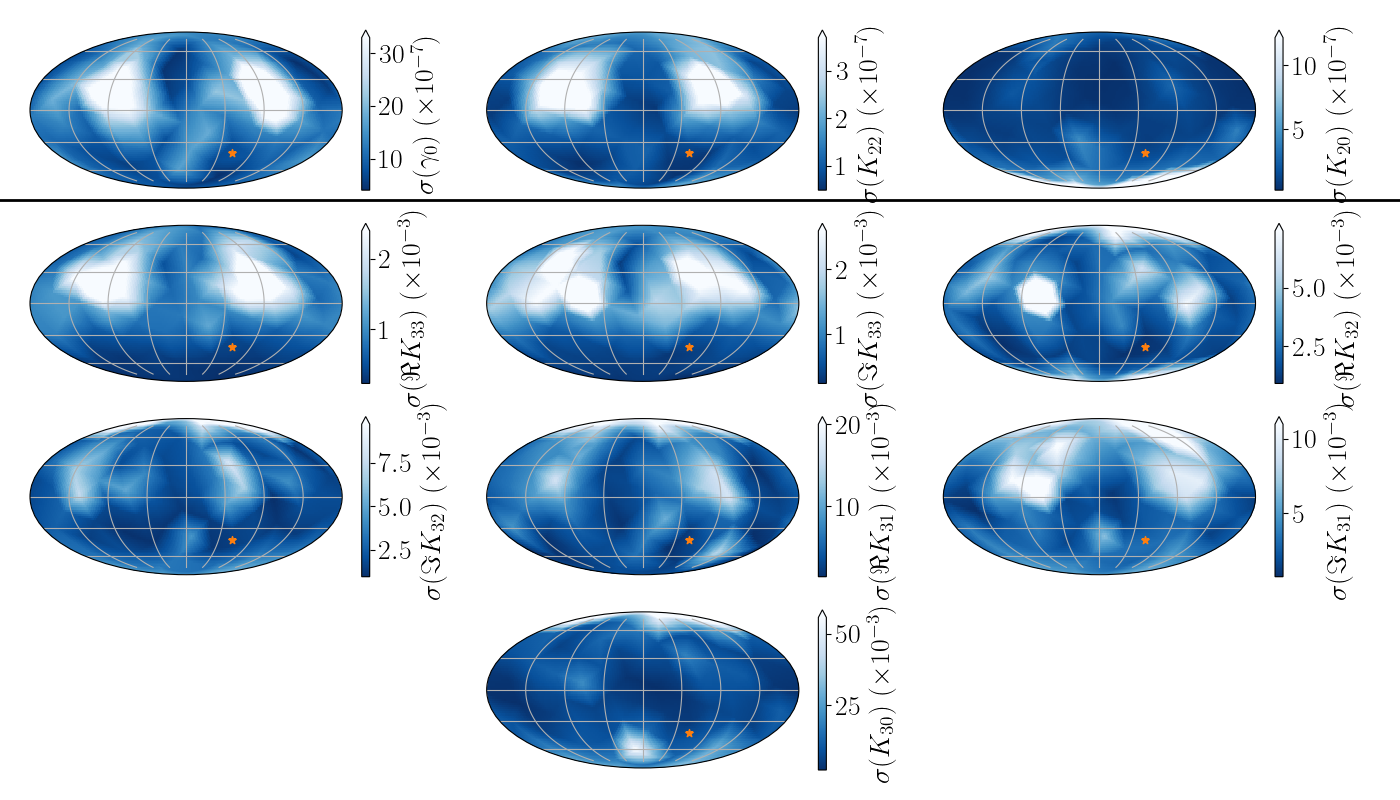
\includegraphics[width=0.8\textwidth]{figs/spin-pole}
  \caption{$1\sigma$ uncertainties for the first-order parameters (\textit{top}) and second-order (\textit{bottom}) as a function of the initial direction of spin in the inertial frame. All maps are made in the Mollweide projection. The orange star indicates the reference spin pole. Green dots are the sampled spin pole directions. The red contours enclose regions above the strong uncertainty threshold on $\sigma_\rho / \rho$. The weak threshold is never exceeded. Beyond the $\pm \unit Z$ increase in uncertainty, there is also increased moment uncertainty for $\pm \unit Y$.}
  \label{fig:scan-spin}
\end{figure*}

Figure \ref{fig:scan-spin} depicts increased moment uncertainty for initial spin pole $\bm \Omega_0 \parallel \unit Z$, as did the density uncertainty discussed in the main text. $\sigma(K_{20})$ especially exhibits this increase. However, many other moments also exhibit increased uncertainty for $\bm \Omega_0 \parallel \pm \unit Y$. This pattern is explained by the tidal torque equation (equation \ref{eqn:tidal-torque}). By plugging in values for the Euler angles, $\bm z \parallel \unit Z$ and $\bm z \parallel \unit Y$ at perigee lead to $\bm \tau \propto K_{22} \unit z$ to first-order, and $\bm \tau \parallel \unit X$ at perigee leads to $\bm \tau = 0$ to first-order. $\bm \tau \parallel \unit z$ implies that only the period of the asteroid is changed, not its spin pole direction. In the case of $\bm \Omega_0 \parallel \unit Z$, we therefore expect $\bm \Omega \parallel \unit Z$ throughout the encounter so that the asteroid does not tumble after the flyby. As discussed in the main text, tumbling allows precise constraints on $K_{2m}$, so that reduced tumbling results in greater uncertainty.

We may understand the case of $\bm \Omega_0 \parallel \unit Y$ by the approximation that $\bm \tau$ is small until perigee, so that the direction of $\bm \Omega$ is unchanged. Insofar as this assumption is accurate, the behaviour of $\bm \Omega_0 \parallel \unit Y$ will be similar to that of $\bm \Omega_0 \parallel \unit Z$, explaining the increased moment uncertainty in this region. This argument breaks down for $\bm \Omega_0 \parallel \unit X$, because here $\bm \tau = 0$, and torque is dominated by non-perigee effects. This may explain why there is no increased uncertainty near $\bm \Omega \parallel \unit X$.


\subsection{Observational uncertainty}
\label{sec:scan-uncertainty}
Two parameters, $\sigma_\theta$ and $\sigma_P$, govern the observational uncertainty of the data set. These parameters are defined in section \ref{sec:uncertainty}; $\sigma_\theta$ represents the standard deviation of the angle between the true spin pole and the observed spin pole, while $\sigma_P$ represents the standard deviation of the rotational period. Rather than explore the full space spanned by these two values, we fix one and allow the other to vary to better assess whether uncertainty in spin pole or uncertainty in period more strongly affects uncertainty. This dependence is displayed in figure \ref{fig:scan-theta}. More precisely, we can ask if some error $\bm {\delta}_\omega$ is added to angular velocity $\bm \omega$, does it affect results more strongly if it is parallel to $\bm \omega$ (affects the period) or perpendicular (affects the spin pole direction)?

Let $\delta = |\bm{\delta}_\omega| / |\bm \omega|$ and $\delta \ll 1$. Then if $\bm {\delta}_\omega \parallel \bm \omega$, it decreases the period $P_\omega$ by $P_\omega \delta$. This is a fractional change in period of $\delta$. If $\bm {\delta}_\omega \perp \bm \omega$, then the spin pole angle changes by $\delta$ radians.

Comparing the $\sigma_P / P$ (fractional change in period) and $\sigma_\theta$ (spin pole angle) columns of figure \ref{fig:scan-observational}, one can see that a given value of $\sigma_\theta$ contributes a much smaller moment uncertainty than the same value of $\sigma_P/ P$. This is also visible in figure \ref{fig:net-uncertainty} for the lumpy model. In other words, if $\bm {\delta}_\omega \perp \bm \omega$ using the symbols defined above, then $\delta$ can be large. But if $\bm{\delta}_\omega  \parallel \bm \omega$, then $\delta$ must be very small. Period precision is therefore more vital than spin pole direction precision when it comes to decreasing density distribution uncertainties.


% \subsection{Cadence}
% \label{sec:scan-cadence}

% The time between observations of asteroid angular velocity, or cadence, may vary depending on the observational schedule of the observing telescopes and the path of the asteroid through the sky.  We measure how the posterior uncertainty $\sigma(K_{\ell m})$ varies with cadence ranging from two minutes to one hour in figure \ref{fig:scan-cadence}.

% Figure \ref{fig:scan-cadence} displays little dependence of uncertainty on cadence $\Delta t$ for $\Delta t \lesssim 40$ min. We also see flaring of uncertainty for very large cadence, largely driven by the paucity of data points. However, uncertainty dramatically increases for many parameters at about $\Delta t = 30-40$ min, a time scale which is likely characteristic of the asteroid system.  We name this rough cadence limit $T_\text{cad}$. $T_\text{cad}$ is also the location at which the $\sigma(K_{3m}$ threshold is crossed for all second-order moments except $K_{30}$, which exceeds the uncertainty threshold at $\Delta t \approx 5$ min.

% We expect this $T_\text{cad}$ to be a function of two dynamical time scales of the system: the rotational period of the asteroid $P_\omega$ and the dynamical time scale of the orbit (the latter can be estimated in multiple ways, since both $r_p / v_\infty$ and $v_\infty r_p^2 / \mu_\mathcal{B}$ have units of time and may be relevant). How these time scales affect $T_\text{cad}$ is discussed in appendix \ref{app:cadence-tests}.

% Figure \ref{fig:scan-cadence} shows that as long as $\Delta t < T_\text{cad}$ is achieved, the influence of cadence on $\sigma$ is minimal, but shorter cadence leads to lower uncertainties.



\subsection{Perigee gap}
\label{sec:scan-gap}
In certain circumstances, spin data might not be able to be captured for a close encounter at perigee. The asteroid might dip below the horizon, or it might pass too close to the sun to be observed. The resulting gap in data is intended to be captured by the $T_\text{gap}$ parameter of figure \ref{fig:scan-observational}, which deserves to be more fully defined.

We mask the perigee of the counter by removing a duration $T_\text{gap}$ of data centred on the perigee, where $T_\text{gap}$ ranges from 0 to 3 hours. To prevent lack of precision induced by lower amounts of data when $T_\text{gap}$ is large, we always cut 3 hr$-T_\text{gap}$ from the data set, half from the beginning and half from the end, so that each data set produced for all $T_\text{gap}$ has the same size. We cut around the perigee because tidal torque is the greatest at perigee, and we expect that part of the data set to be most valuable. Indeed, figure \ref{fig:scan-observational} shows that $K_{3m}$ especially are more uncertain for $T_\text{gap} \gtrsim 1.5$ hr. However, figure \ref{fig:net-uncertainty} shows that $T_\text{gap}$ never increases density uncertainty above the thresholds, indicating that large amounts of data can be cut without compromising the methodology.